% !TEX root = main.tex
%%%%%%%%%%%%%%%%%%%%%%%%%%%%%%%%%%%%%%%%%%%%%%%%%%%%%%%%%%%%%%%%%%%%%%%%%%%%%%%%
% Document Header
%%%%%%%%%%%%%%%%%%%%%%%%%%%%%%%%%%%%%%%%%%%%%%%%%%%%%%%%%%%%%%%%%%%%%%%%%%%%%%%%
\documentclass[conference]{IEEEtran}
\IEEEoverridecommandlockouts
\usepackage{cite}
\usepackage{amsmath,amssymb,amsfonts}
\usepackage{algorithmic}
\usepackage{graphicx}
\usepackage{textcomp}
\usepackage{xcolor}
\usepackage[section]{placeins}
\def\BibTeX{{\rm B\kern-.05em{\sc i\kern-.025em b}\kern-.08em
    T\kern-.1667em\lower.7ex\hbox{E}\kern-.125emX}}
%\usepackage[pdftex,
%            bookmarksopen=true,
%            colorlinks,
%            linkcolor={black},
%            citecolor={black},
%            urlcolor={black}]{hyperref}
\newcommand{\href}[2]{#2}

%%%%%%%%%%%%%%%%%%%%%%%%%%%%%%%%%
% The Double-blind Review Command
%%%%%%%%%%%%%%%%%%%%%%%%%%%%%%%%%
%\newcommand{\doubleblind}[2]{#1} % Use this command for final submission
\newcommand{\doubleblind}[2]{#2} % Use this command for review submission

%%%%%%%%%%%%%%%%%
% Custom Commands
%%%%%%%%%%%%%%%%%
\newcommand{\fix}[1]{\textcolor{red}{#1}}
\newcommand{\pkg}[1]{{\tt #1}}
\newcommand{\indf}[1]{$\rightarrow$~\textcolor{blue}{#1}}

%%%%%%%%%%%%%%%%%%%%%%%%%%%%%%%%%%%%%%%%%%%%%%%%%%%%%%%%%%%%%%%%%%%%%%%%%%%%%%%%
% Document Body
%%%%%%%%%%%%%%%%%%%%%%%%%%%%%%%%%%%%%%%%%%%%%%%%%%%%%%%%%%%%%%%%%%%%%%%%%%%%%%%%
\begin{document}

%%%%%%%%%%%%%%%%%%%%%%%%%%%%%%%%%%%%%
% Title & First-Page Acknowledgements
%%%%%%%%%%%%%%%%%%%%%%%%%%%%%%%%%%%%%
\title{GPU Lifetimes on Titan Supercomputer: \\ Survival Analysis and Reliability%
\doubleblind{\thanks{This work was sponsored by the U.S. Department of Energy's
Office of Advanced Scientific Computing Research. This manuscript has been
authored by UT-Battelle, LLC under Contract No. DE-AC05-00OR22725 with the U.S.
Department of Energy. The United States Government retains and the publisher,
by accepting the article for publication, acknowledges that the United States
Government retains a non-exclusive, paid-up, irrevocable, world-wide license to
publish or reproduce the published form of this manuscript, or allow others to
do so, for United States Government purposes. The Department of Energy will
provide public access to these results of federally sponsored research in
accordance with the DOE Public Access Plan
(http://energy.gov/downloads/doe-public-access-plan).}{}}}

%%%%%%%%%
% Authors
%%%%%%%%%
\author{\doubleblind{
\IEEEauthorblockN{1\textsuperscript{st} George Ostrouchov}
\IEEEauthorblockA{\textit{Computer Science and Mathematics Division}\\
\textit{Oak Ridge National Laboratory}\\
Oak Ridge, TN, USA\\
ostroughovg@ornl.gov}
\and
\IEEEauthorblockN{2\textsuperscript{nd} Don Maxwell}
\IEEEauthorblockA{\textit{National Center for Computational Sciences Division}\\
\textit{Oak Ridge National Laboratory}\\
Oak Ridge, TN, USA\\
maxwellde@ornl.gov}
\and
\IEEEauthorblockN{3\textsuperscript{rd} Rizwan Ashraf}
\IEEEauthorblockA{\textit{Department of Electrical Engineering and Computer Science}\\
\textit{University of Tennessee}\\
Knoxville, TN, USA\\
rizwan.ashraf@knights.ucf.edu}
\and
\IEEEauthorblockN{4\textsuperscript{th} Christian Engelmann}
\IEEEauthorblockA{\textit{Computer Science and Mathematics Division}\\
\textit{Oak Ridge National Laboratory}\\
Oak Ridge, TN, USA\\
engelmannc@ornl.gov}
\and
\IEEEauthorblockN{5\textsuperscript{th} James Rogers}
\IEEEauthorblockA{\textit{National Center for Computational Sciences Division}\\
\textit{Oak Ridge National Laboratory}\\
Oak Ridge, TN, USA\\
jrogers@ornl.gov}}{}}

\maketitle

%%%%%%%%%%%%%%%%%%%%%%%%%%%%%%%%%%%%%%%%%%%%%%%%%%%%%%%%%%%%%%%%%%%%%%%%%%%%%%%%
% Abstract
%%%%%%%%%%%%%%%%%%%%%%%%%%%%%%%%%%%%%%%%%%%%%%%%%%%%%%%%%%%%%%%%%%%%%%%%%%%%%%%%
\begin{abstract}
This system was \#1 in the world for a very long time, and has remained
a critically important computer system. It defied scale with 18,688
individual compute nodes, and delivered tens of billions of computing
hours to DOE mission-critical programs for nearly 7 years. 

\end{abstract}

%%%%%%%%%%%%%%%%%%%%%%%%%%%%%%%%%%%%%%%%%%%%%%%%%%%%%%%%%%%%%%%%%%%%%%%%%%%%%%%%
% Keywords
%%%%%%%%%%%%%%%%%%%%%%%%%%%%%%%%%%%%%%%%%%%%%%%%%%%%%%%%%%%%%%%%%%%%%%%%%%%%%%%%
\begin{IEEEkeywords}
GPU, reliability, supercomputer, NVIDIA, Cray, large-scale systems,
Kaplan-Meier survival, Cox regression
\end{IEEEkeywords}

%%%%%%%%%%%%%%%%%%%%%%%%%%%%%%%%%%%%%%%%%%%%%%%%%%%%%%%%%%%%%%%%%%%%%%%%%%%%%%%%
% Sections
%%%%%%%%%%%%%%%%%%%%%%%%%%%%%%%%%%%%%%%%%%%%%%%%%%%%%%%%%%%%%%%%%%%%%%%%%%%%%%%%

%%%%%%%%%%%%%%
% Introduction
%%%%%%%%%%%%%%
\section{Introduction}
\label{sec:intro}
\fix{Dropped Jim's initial email here.}
The Cray XK7 Titan is rapidly nearing its decommissioning date for
DOE/ASCR. The last production runs will be in July of this year, and
then we will stop services, clean up a few things and turn it off. 
 
This system was \#1 in the world for a very long time, and has remained
a critically important computer system. It defied scale with 18,688
individual compute nodes, and delivered tens of billions of computing
hours to DOE mission-critical programs for nearly 7 years. 
 
This was quite an interesting machine from a reliability perspective.
We were forced to execute three very significant rework cycles, two on
the mechanical assembly affecting the PCIe connector from the GPU
daughtercard to the motherboard, and more recently, a replacement of
about 11,000 GPU assemblies because of a failing resistor on a printed
circuit board. 
 
We have conducted a good bit of statistical analysis on the failure
rates of these GPU assemblies, but I want to propose a different topic
that I have not seen for other/similar systems.  I want to complete
the statistical analysis of the failure rates as we near end of life,
looking for the opposite side of the “bathtub curve”.  There is
specific decay associated with the electronic components where, as
these products age, they will eventually fail thresholds for guard
band margin and other things. In a lot of cases, they will just fail
as well. 
 
This machine is quite large, was very important to many people, and I
think this analysis could be very intriguing. 
 
I am looking for help, very specifically with the statistics portion
of this, i.e. what do the failure rates for specific components look
like? What distributions do those failure rates follow? How could
appropriate models extrapolate failure rates beyond the end of service
date (the dotted lines…) ? 
 
I have submitted an abstract to a Cray-focused user group and workshop
on this topic, and it has been accepted.  I would like to execute this
statistical analysis and generate a short presentation (30 minutes)
and a short paper (4-8 pages is a likely target).  Presentation is
targeted for May 7-9 (TBD). An initial/working version of the paper
would be due earlier. If we miss that target (April 12), no big
deal. We can finish on a similar schedule as the presentation.  I have
all of the raw data for the component failures, and need the
statistical help to complete the analysis. 
 
Because there is a huge swing in the failure rates of the GPUS from
2016/17 when the resistor problem escalated rapidly out of control, it
is statistically interesting, where we inject fresh material in to an
existing machine. We’d likely want to categorically separate new GPU
assemblies from old and could track the early life failures from those
new 11,000 parts versus the continued failure of the remaining 6000. 
 
George, Christian-  any interest in this? Barney gave it a thumbs
up. I think this is a timely and very interesting topic. 

\fix{Need a description of Titan GPU events timeline. Jim or Don?}


%%%%%%%%%%%%%%
% Related Work
%%%%%%%%%%%%%%
% !TEX root = main.tex
%%%%%%%%%%%%%%%%%%%%%%%%%%%%%%%%%%%%%%%%%%%%%%%%%%%%%%%%%%%%%%%%%%%%%%%%%%%%%%%%
% Related Work
%%%%%%%%%%%%%%%%%%%%%%%%%%%%%%%%%%%%%%%%%%%%%%%%%%%%%%%%%%%%%%%%%%%%%%%%%%%%%%%%
\section{Related Work}
\label{section:related}

Prior work in investigating Titan's reliability includes a significant amount of work that covers different aspects. However, it did not investigate the atypical failure mode discussed in this paper and failure data over the full lifetime of the system.

Tiwari et al~\cite{Tiwari15Experience,7056044} analyzed the types of GPU errors on Titan and on a GPU cluster at Los Alamos National Laboratory. It also used neutron beam experiments at the Los Alamos Neutron Science Center and at Rutherford Appleton Laboratories to further understand GPU soft errors caused by neutron radiation triggered upsets (bit flips and timing errors).
%
Tiwari et al~\cite{10.1145/2807591.2807666} further analyzed the types of GPU errors on Titan, including software/firmware related errors and failures, ECC double-bit errors, and GPU ``off the bus'' and ECC page retirement events. This work observed a ECC double-bit mean-time between errors (MTBE) of about 160 hours, or about one per week, with 86\% in GPU memory and the rest in the GPU register file. The experienced GPU ``off the bus'' events were caused by a system integration issue that was fixed and not an inherent GPU or GPU memory architecture flaw.
%
Nie et al.~\cite{7446091,nie17characterizing,nie18machine} characterized the soft error behavior of Titan's GPUs in relation to temperature and power consumption to predict their increased occurrence by correlating data in temporal and spatial domains and using machine learning models. The work primarily focused on correctable single-bit errors.
%
Tiwari et al. and Nie et al. did not address the atypical failure mode discussed in this paper. It also only used Titan error and failure data from June 2013 to February 2015, excluding early failures and the failure mode discussed in this paper (which occurred after February 2015).

Zimmer et al.~\cite{8665764} developed a new job scheduling strategy for Titan to counter the GPU failures discussed in this paper and to improve system utilization and productivity. The solution used reordering of compute nodes for resource allocation, scheduling larger jobs on more reliable and smaller jobs on less reliable nodes.

Ezell~\cite{osti_1086655} created a general understanding of Titan's interconnect failures using an application to stress test Titan's Gemini interconnect.
%
Work by Kumar et al.~\cite{kumar18understanding} analyzed Titan's interconnect faults, errors and congestion events to improve interconnects resilience and congestion resolution methods. The results show that the magnitude of interconnect errors is very high with an uneven distribution across different types of links is uneven. They also show that congestion is highly frequent and bursty.
%
Gupta et al.~\cite{7266836} investigated the spatial and temporal properties of failures on Titan and their impact on resilience mechanisms and the implications for efficient system operation.
%
Gupta et al.~\cite{gupta17failures} also performed a study covering five supercomputers at Oak Ridge National Laboratory, including Titan, that concentrated on developing an understanding of which and how many errors and failure occur in supercomputers over multiple generations and over their years of operation. This work resulted in a lot of lessons learned, including that the mean-time between failures (MTBF) can change drastically and non-monotonically over time.
%
Meneses et al.~\cite{Meneses15Analyzing} analyzed the interplay and workload on Titan using failure and job submission logs. The results indicate that failures depend heavily on workload.

Bautista-Gomez et al.~\cite{bautista-gomez16reducing} used failure data from Titan to adapt the checkpoint frequency to the current reliability of the system using dynamic checkpointing.
%
Tiwari et al.~\cite{6903564} also used failure data from Titan and exploited temporal locality in the data to adapt the checkpoint frequency to the current reliability of the system using lazy checkpointing.
%
Both approaches, Bautista-Gomez et al. and Tiwari et al., aim at dealing with the drastically and non-monotonically changing MTBF of Titan to match current system reliability with an efficient recovery strategy.

Other work in characterizing supercomputer faults, errors and failures focused on the various systems deployed around the world, primarily at US Department of Energy laboratories.
%
Di et al.~\cite{8809553} developed an in-depth understanding of the failure characteristics of the IBM Blue Gene/Q Mira system at Argonne National Laboratory. This work showed that 99.4\% of job failures were due to user behavior, such as errors in the code or misconfiguration. Martino et al.~\cite{6903615} characterized the errors and failures of the Blue Waters Cray XE6/XK7 system at the National Center for Supercomputing Applications (NCSA), at the University of Illinois at Urbana-Champaign. The results showed that 74.4\% of system-wide outages in Blue Waters were caused by software. Blue Waters's XK7 partition had the same architecture as Titan, but did not experience the same GPU failure mode detailed in this paper.


%%%%%%%%%%%%%%%%%%%%%%%%%%%%%%%%%%%
% Data Collection and Preprocessing
%%%%%%%%%%%%%%%%%%%%%%%%%%%%%%%%%%%
\section{Data Collection and Preprocessing}
\label{sec:data}
\fix{Don's section}
Data on GPU life times is constructed from two sources: inventory runs
and failure event records (DBX and Off the Bus).

An inventory of GPU serial numbers and their locations is recorded
each time the system boots. This typically occurs once every few days but
can be as frequent as a few times per day. An inventory at boot time
typically occur-rs over a span of \fix{??} minutes. A separate file is
produced at each boot time.

The DBE and Off The BUS events are also recorded separately from boot
time inventories. This is recorded as . . . files.

Initial processing updates an inventory by checking the Serial Number
(SN) and Location of each GPU and creating or updating a separate
record for each contiguously observed SN-Location combination.

Figure~\ref{fig:inventory} shows inventory times that appear in the
data grouped into three categories. Only the time axis is relevant
here as the vertical scatter within each category is added only to
control overplotting. It appears that the early period before mid 2015
has relatively few inventories taken, inventory frequency increases
through the end of 2016, then it decreases slightly and becomes
steady. There is also a nearly year-long gap in Off The BUS
occurrences. After removing the OTB and DBE dates, the time
distribution becomes fairly uniform. This suggests that the OTB and
DBE times are independent of the boot time inventories.

\fix{Don, the figures bring more questions: Are the OTB and DBE events
recorded independently of the boot time inventories? The figures are
the distributions of referenced times in the data. Separate graphs are
done for OTB and DBE events, for general life span insert and remove
dates, and again after removing the OTB and DBE times. After the
removal, the times are fairly uniformly distributed. Does that mean
that boot time inventories are done fairly uniformly?}

\begin{figure}[bth]
  \centering
  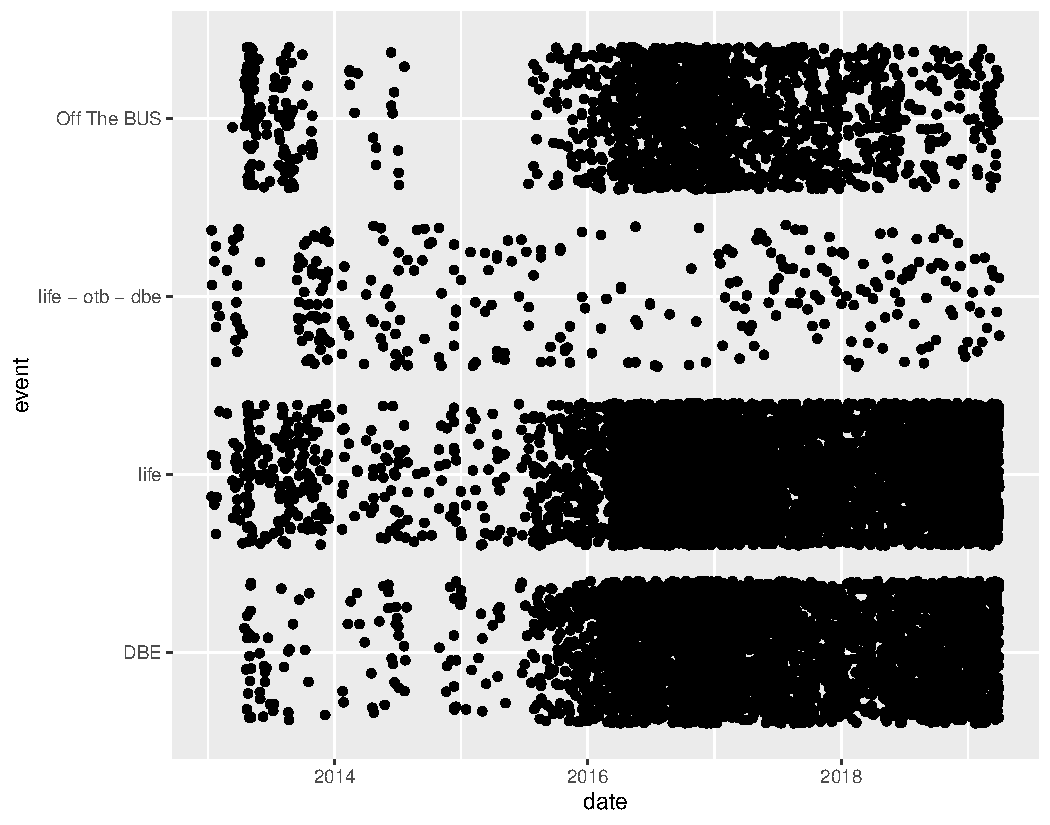
\includegraphics[width=\textwidth]{inventory_times.pdf}
  \caption{Inventory times in all of the data separated into ``DBE''
    and ``Off The BUS'' failure events, and observed insert-remove
    times as ``life'' and again after removing the failure times as
    ``life - otb - dbe''. Vertical point jitter is applied to each to
    mitigate overplotting effects.}
  \label{fig:inventory_dates}
\end{figure}
\begin{figure}[bth]
  \centering
  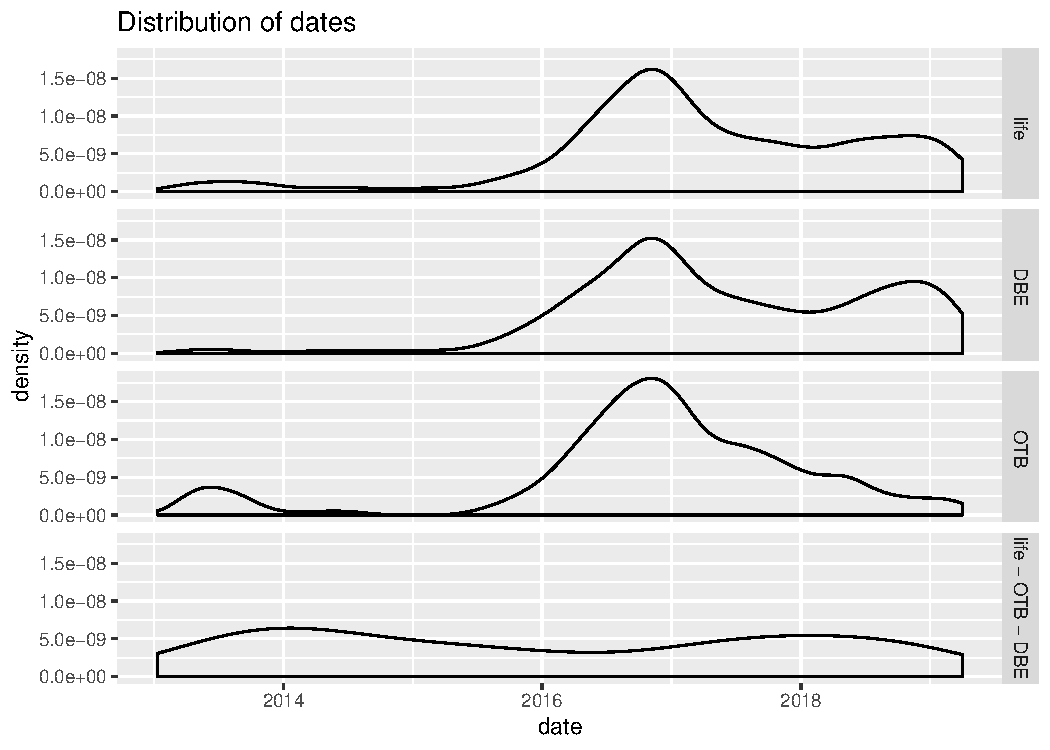
\includegraphics[width=\textwidth]{inventory_density.pdf}
  \caption{Inventory times density in all of the data separated into
    ``DBE'' and ``Off The BUS'' failure events, and observed
    insert-remove times as ``life'' and again after removing the
    failure times as ``life - otb - dbe''. Compare to jittered dates
    in Fig.~\ref{fig:inventory_dates}.}
  \label{fig:inventory_density}
\end{figure}


%%%%%%%%%%%%%%%%%%%%%%%%%%%%%%%
% Viewing and Cleaning the Data
%%%%%%%%%%%%%%%%%%%%%%%%%%%%%%%
\section{Viewing and Cleaning the Data}
\label{sec:clean}
\fix{George's section: The two views of GPU life: by SN and by
  location, its use in cleaning data, etc.}

As we need to recover durations from this data, correct processing
involves time adjustments for switching between daylight saving time
and standard time. We perform this by setting a reference time zone
(Eastern time) and converting all date-times from strings into
date-time variables \fix{(is there a name for this?)} with the R
\pkg{lubridate} package \cite{lubridate}, which enables appropriate
date arithmetic.

\fix{Other processing:} enable missing values, and create some new
variables. The event is “life” when both insert and remove are
present, “life0” when insert = remove, otherwise it is whatever string
is in insert, which is “DBE” or “Off The BUS”. Also separate location
into its components and fill in (repeat) serial numbers and locations
for all records.

Reduce to only “life” records and mark them with ending DBE, OTB,
“out”, or none events. The result is just insert and remove with event
marks to indicate DBE or OTB or “out” (last seen). bad indicates that
a DBE or OTB occurred yet the GPU was not taken out. For a first cut,
keep the bad ones in. Also keep duration to later aggregate into full
life times.

Next, aggregate into one record per serial number with total life time
and first insert time. For proper censoring treatment: Indicate if
event occurred or still in service: out = fail, dbe = fail, otb =
fail, NA = right censored (still in service). Add some other
variables, such as GPU in single location or moved one or more times,
mark new\_batch group, etc. to use in modeling later.

To get some intuition for the GPU lifetimes on Titan, we give two views of
a hundred GPUs (Figure~\ref{fig:gpuview}) and a hundred locations
(Figure~\ref{fig:locview}). The GPU view is ``by serial number'' that
shows when each GPU was installed and removed at various locations as
well as its DBE and OTB events. The second view by location, shows
when different GPUs were installed and removed at a location, and
their OTB and DBE events.
\begin{figure}[ht]
  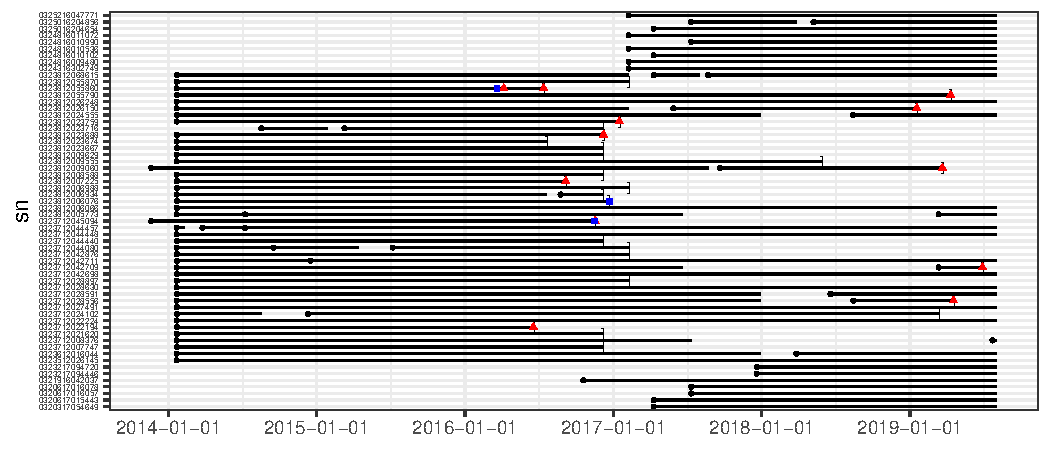
\includegraphics[width=6in]{figs/sample_sn.pdf}
  \caption{GPU serial number view of life and failures. Legend: black
    dots are installs, black lines are lifetimes at installed
    location, blue squares are OTB events, red triangles are DBE
    events, and black ] are ``last seen'' events.}
  \label{fig:gpuview}
\end{figure}
\begin{figure}[ht]
  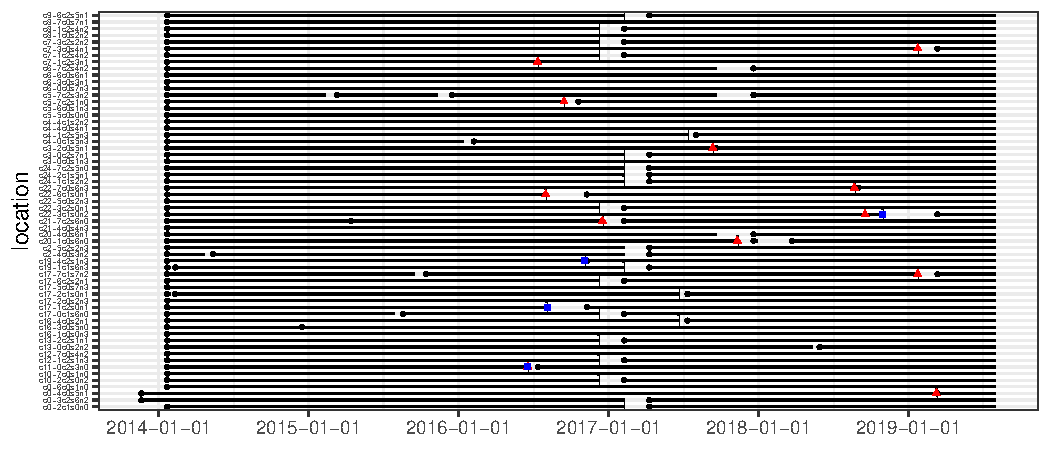
\includegraphics[width=6in]{figs/sample_loc.pdf}
  \caption{GPU location view of life and failures.  Legend: black
    dots are installs, black lines are lifetimes at installed
    location, blue squares are OTB events, red triangles are DBE
    events, and black ] are ``last seen'' events.}
  \label{fig:locview}
\end{figure}
The serial number view clearly shows the two batches and the more
frequent OTB and DBE events in the old batch. It is also clear from
this view that most new GPUs stay at the initial install location
whereas the old GPUs were occasionally reinstalled at new locations.
The location view shows that each location was operational almost all
the time with small gaps when GPUs were changed out.

\fix{Were the GPUs swapped out as a blade or were individual GPUs
  swapped on a blade?}


%%%%%%%%%%%%%%%%%%%%%%%%%%%%%%%%
% Time Between Failures Analysis
%%%%%%%%%%%%%%%%%%%%%%%%%%%%%%%%
% !TEX root = main.tex
%%%%%%%%%%%%%%%%%%%%%%%%%%%%%%%%%%%%%%%%%%%%%%%%%%%%%%%%%%%%%%%%%%%%%%%%%%%%%%%%
% Time Between Failures Analysis
%%%%%%%%%%%%%%%%%%%%%%%%%%%%%%%%%%%%%%%%%%%%%%%%%%%%%%%%%%%%%%%%%%%%%%%%%%%%%%%%
\section{Time Between Failures Analysis}
\label{section:tbf}

\begin{figure}[bt]
  \begin{center}
    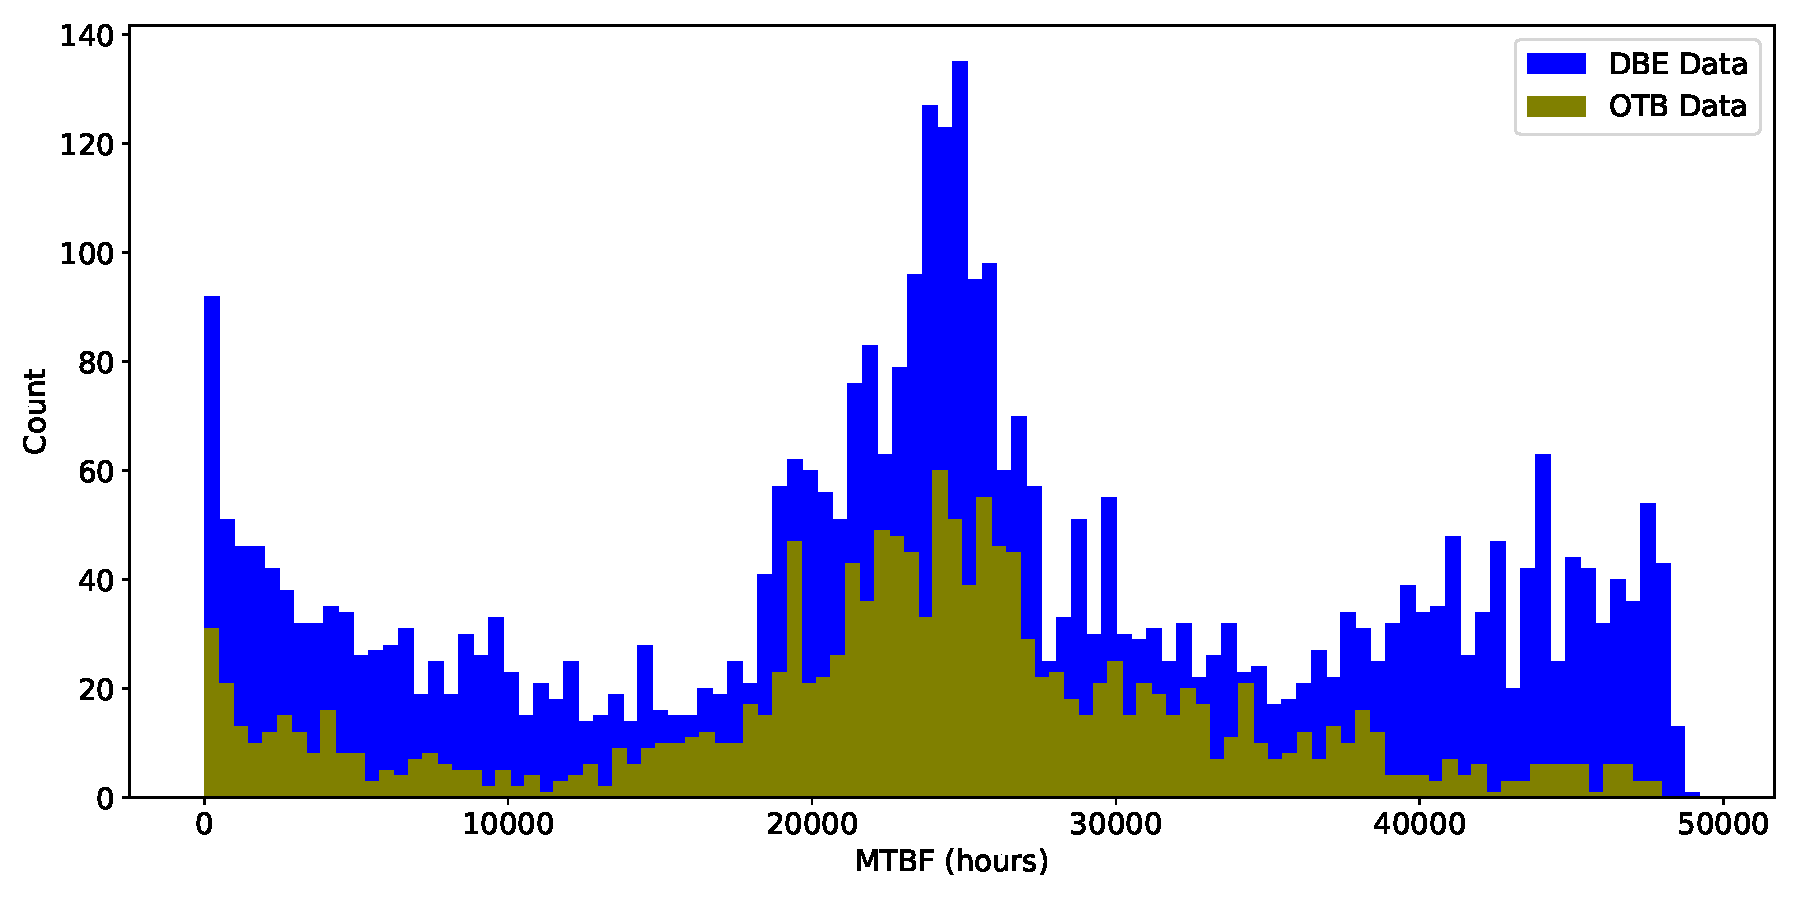
\includegraphics[width=\columnwidth]{figs/MTBF_GPUwise.pdf}
  \end{center}
  \caption{Distribution of MTBFs due to DBEs and OTBs across all GPUs.}
  \label{fig:Device_MTBFs}
\end{figure}

Using the processed data, we analyze the inter-arrival times between the DBE and OTB events. 
This analysis is done at the device level and the system level. 
It provides important insights into the reliability of large-scale machines, where the 
failure rate of an individual device is significantly different from the overall reliability
of the machine.  

A histogram of MTBFs measured across GPUs which had at least one failure event is shown 
in Figure~\ref{fig:Device_MTBFs}. This is a practical assessment of device reliabilities 
as opposed to those provided in the device datasheet. The failures are tracked using the
SN of the GPUs even though a GPU might have been placed at different locations in the 
machine during its lifetime. The time to the first failure on a device is measured by taking
the insert time as the reference point, whereas, a simple difference is taken for subsequent
failures. It can be noticed that MTBFs due to DBE and OTB failures of most GPUs are clustered around 
25,000 hours or 2.8 years. Apart from the center cluster, a significant portion of GPUs has a very 
low MTBF (less than 1.5 hours) due to both DBE and OTB failures. This shows that a device 
can see a failure immediately after it is put into service or multiple events are caused due 
to a single root cause. On the other end of the spectrum, a noticeable portion of GPUs have very high
MTBFs due to DBE failures. This indicates that most GPUs see a single DBE during their lifetime.
Apart from this behavior, the distribution of MTBF due to DBE events looks very similar to that due 
to OTB events. Overall, it can be noted from Figure~\ref{fig:Device_MTBFs} that the number of recorded 
DBE events is significantly higher than the OTB events. 

\begin{figure}[bt]
  \begin{center}
    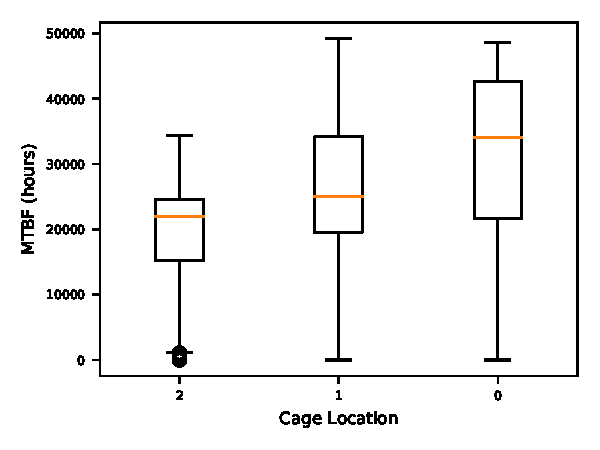
\includegraphics[width=\columnwidth]{figs/MTBF_CageWise.pdf}
  \end{center}
  \caption{MTBFs due to either DBEs or OTBs across the GPUs located in different cages.}
  \label{fig:CageWise_MTBFs}
\end{figure}

\fix{Figure~\ref{fig:CageWise_MTBFs} shows temperature effect clearly. Should we move this 
result to later in the paper?}

\begin{figure}[bt]
  \begin{center}
    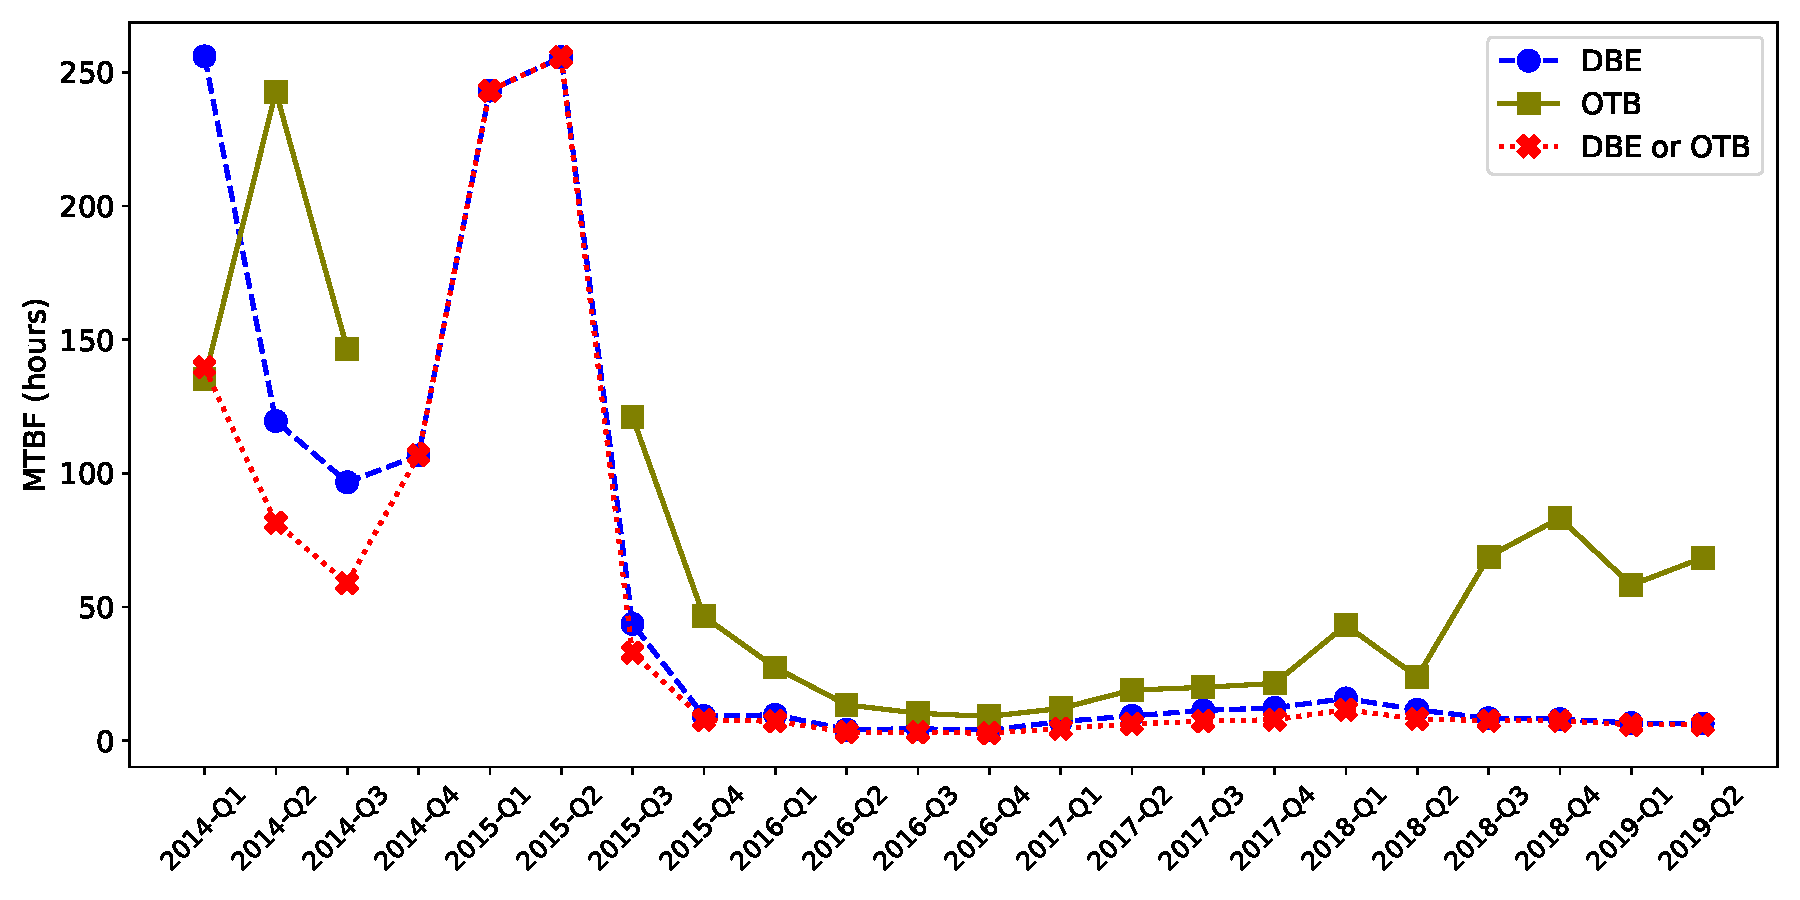
\includegraphics[width=\columnwidth]{figs/MTBF_quaterly_sys.pdf}
  \end{center}
  \caption{Variation of system-wide MTBF over the lifetime of the machine (time is segmented into quarters, 
i.e., January through March is Q1 and so on).}
  \label{fig:MTBF_sys}
\end{figure}

Although individual device MTBFs provide important insights into the varying failure rates
observed across the machine. It is worthwhile to perform a system-wide MTBF analysis since 
most high-performance computing applications use a significant number of GPUs in parallel. 
In the following analysis, failures occurring across all GPUs are consolidated and time between failures
is calculated. The old and new GPUs are all considered. At any given time, only a fixed number of GPUs
are in operation so any variation in time-between-failures is due to individual device reliabilities.

That said, a single MTBF number does not give an accurate picture of this machine.
With many GPU relocations and replacements across the machine over its lifetime, it is 
best to consider the variation of MTBF across fixed periods. Herein, we calculate 
the mean of time-between-failures across three months. Figure~\ref{fig:MTBF_sys}
clearly shows the considerable change in system-wide MTBF from one period to another. 
The observation of the MTBF trend shows the different phases which the machine went through. 
For example, when considering failure due to both DBE and OTB events more than 4X drop in MTBF is 
noted from 2015-Q3 to 2015-Q4 (note, MTBF of earlier quarters was significantly higher and is not 
included in the figure to better visualize various change points). This period marked the start of 
a rapid decline in system-wide MTBF until 2016-Q4. The rapid rise of the number of failures before this 
quarter can be seen in Figure~\ref{fig:NumFails_sys}. When GPU replacements start to take place in late 
2016, it triggers an increase in MTBF. However, this change only lasts until 2018-Q1, when we see another 
downward trend of system MTBF. Incidentally, 2018-Q1 also marks the completion of all GPU replacements. 
So the upward trend noted in the period from 2016-Q4 to 2018-Q1 might be attributed to a portion of the machine 
being unavailable while the reworks were taking place. A single replacement cycle lasted multiple weeks. 
\fix{need to verify how long the replacement took}
There is no definite way to incorporate this unavailability of the machine into MTBF analysis, so it has to
be said that overall there has been an increase in MTBF of the machine due to the replacements. 
For example, before 2017-Q1 MTBF as low as 2.7 hours is noted, whereas the lowest MTBF is 5.9 hours after this 
period. With such huge variations in system MTBF, it is difficult to reliably run applications even while using 
failure recovery approaches such as checkpoint restart, as discussed later on in Section~\ref{section:discussion}. 

The mean-time-between DBE and OTB failures are separately tracked as well in this analysis.
One observation is the drastic increase in mean-time-between OTB failures after the GPU replacements.
This is also evident from the reduction of the absolute number of OTB failures in Figure~\ref{fig:NumFails_sys}.
However, the machine's MTBF is determined by the weakest link and DBE events tend to dictate it.
Even though the replacements helped to increase the MTBF due to DBE events by a factor, the overall system 
reliability is dictated by the components with the most age in the system. There is an upward trend towards 
the end in the number of DBE failures in Figure~\ref{fig:NumFails_sys} which almost all of them are due to 
older GPUs in the system. The old GPUs that occupy a minority portion of the machine after GPU replacements
 and have a disproportionately high number of failures play a major role in determining the state of the 
machine as noted in the next section.

\begin{figure}[bt]
  \begin{center}
    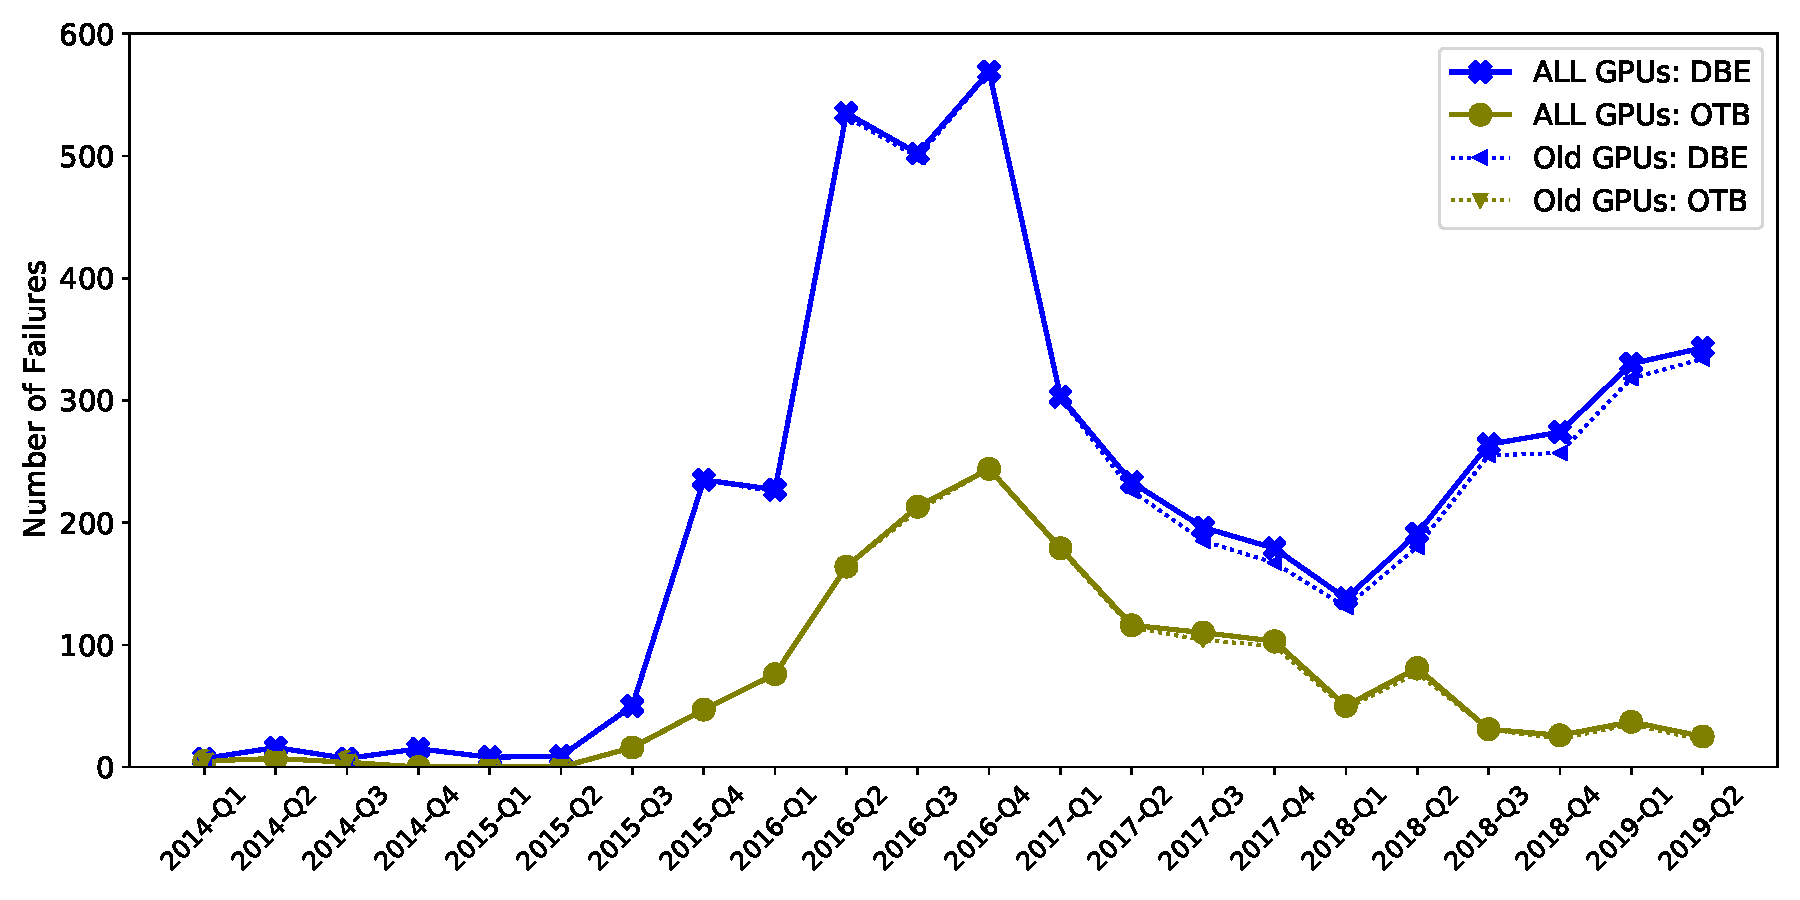
\includegraphics[width=\columnwidth]{figs/NumFailures_Quarterly_newOld.pdf}
  \end{center}
  \caption{The number of DBE and OTB failures observed over the lifetime of the machine.
A distinction is made for GPU failures happening across old GPUs to signify the number 
of failures across the newer GPUs.}
  \label{fig:NumFails_sys}
\end{figure}


%%%%%%%%%%%%%%%%%%%
% Survival Analysis
%%%%%%%%%%%%%%%%%%%
% !TEX root = main.tex
%%%%%%%%%%%%%%%%%%%%%%%%%%%%%%%%%%%%%%%%%%%%%%%%%%%%%%%%%%%%%%%%%%%%%%%%%%%%%%%%
% Survival Analysis
%%%%%%%%%%%%%%%%%%%%%%%%%%%%%%%%%%%%%%%%%%%%%%%%%%%%%%%%%%%%%%%%%%%%%%%%%%%%%%%%
\begin{figure*}
  \centering
  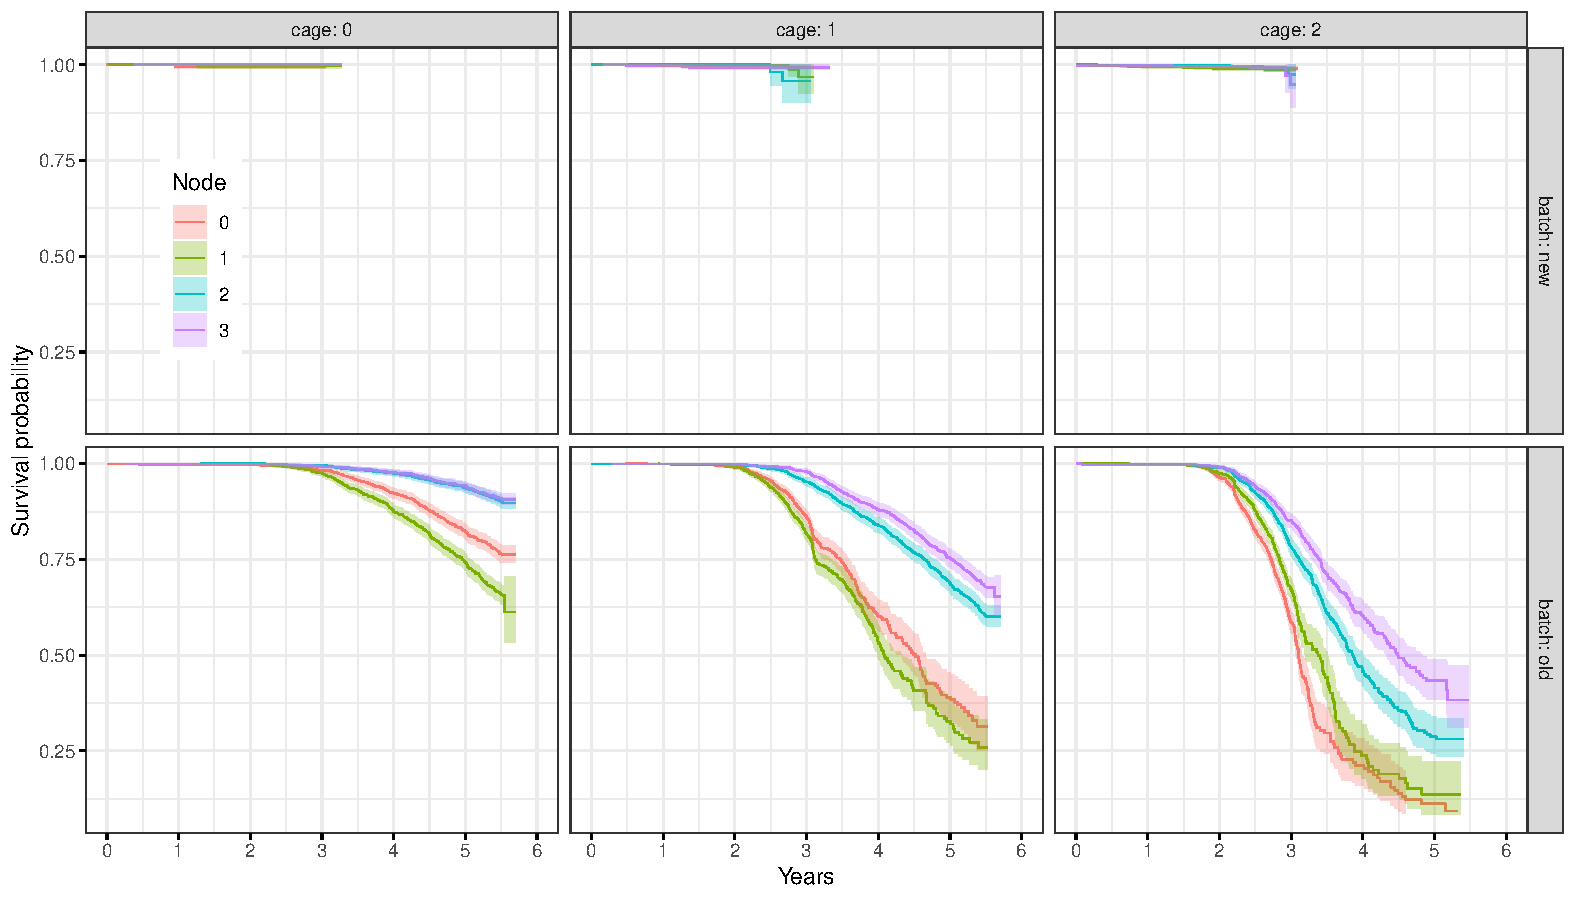
\includegraphics[width=7in]{figs/km_cage-node_a001.pdf}
  \caption{Comparison of the old and new batches, including survival
    differences based on {\tt cage} and {\tt node} GPU locations.}
  \label{fig:km-all-cage-node}
\end{figure*}
\section{Survival Analysis}
\label{section:survival}
\renewcommand{\pkg}[1]{\textsf{#1}}
In this section we apply survival analysis methods (time to event
analysis), which use and combine information across the operational
lifetimes of all GPUs \cite{survival}. For these analyses, we take
apart the location string of each GPU into variables {\em col, row,
  cage, slot, and node} and study the influence of the locations on
the GPU life times. The construction of a GPU life time is more
complex than it initially appears because the units are observed only
at reboot time, because most units were proactively replaced to
prevent failure, and because some units continue in operation after
OTB and DBE events (when a second reboot may be successful).

A unit that experiences at least one OTB or DBE event and is removed
from the system is considered failed and its operation time until the
last seen time is taken as its life time. Although most failed units
experience one of these events at the last seen time, our definition
is not perfect because some units experience OTB or DBE events at a
time different from its last seen time. Such units were relatively few
so we consider this definition of life time as the most pragmatic.

A key concept in survival analysis is censoring, which is about using
information from study subjects whose exact failure times are not
available or that have not failed. This applies to our study because
of proactive GPU replacement before failure, because most units were
still in operation when the system was shut down, and also because
life spans were recorded only at inventory times. We use censoring
concepts on the proactive replacements and units still in operation at
the end. This allows us to use all of the GPU life time data,
including units that did not fail. But we ignore the inspection time
censoring, treating inventory times as exact failure times to reduce
the complexity of this analysis. We expect that because of the volume
of data and length of operation time, this would not make much
difference in our conclusions. However, we are making our data
publicly available and expect that others, especially in the survival
analysis community, will dive deeper.

Kaplan-Meier survival analysis (KM) starts with computing the
probability of survival beyond a given time. It is a nonparametric
technique that makes no specific failure model assumptions, such as
Weibull, Exponential, etc. The technique is able to use censored
observations and can also split the data into subpopulations to
compute separate survival curves.

If $T$ is the random variable of a GPU fail time, then its cumulative
distribution function $F(t) = Pr\{T < t\}$ gives the probability that
a GPU fails by duration $t$. The survival function is its complement
\begin{displaymath}
  S(t) = Pr\{T \geq t\} = 1 - F(t).
\end{displaymath}
It is the probability of being operational at duration $t$.  We use
the R packages \pkg{survival} and \pkg{survminer} for the KM analysis,
which is reported in Figure~\ref{fig:km-all-cage-node}. Within each
{\em batch}, separate survival curves are computed for each {\em cage}
by {\em node} combination. Along with the survival curve estimate,
this analysis provides 95\% confidence region for survival probability
shaded around the curves.
% Inserting figure here so it appears at top of next page
\begin{figure}
  \centering
  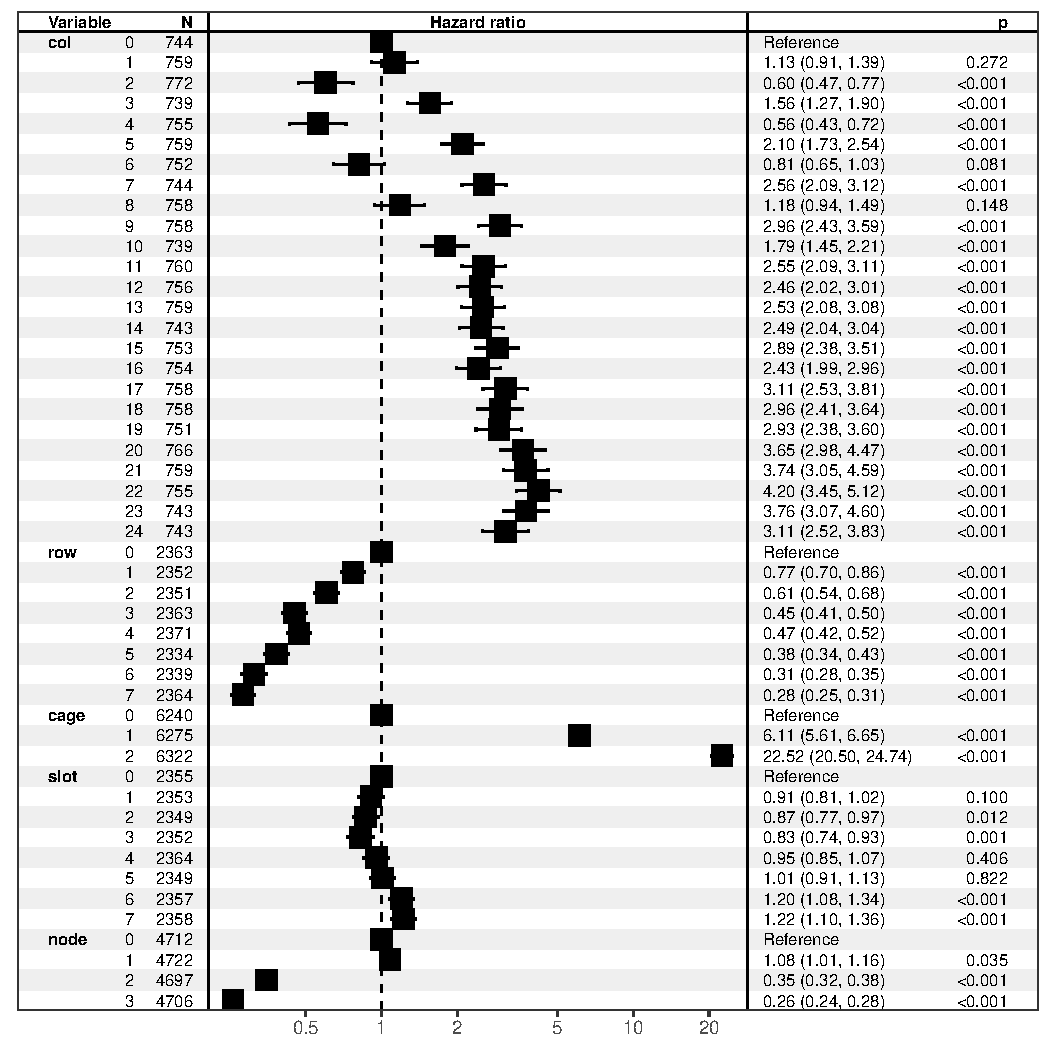
\includegraphics[width=\columnwidth]{figs/cox_o001.pdf}
  \caption{GPU hazard ratios from Cox regression model on {\tt old}
    batch.}
  \label{fig:cox-old}
\end{figure}
\begin{figure}
  \centering
  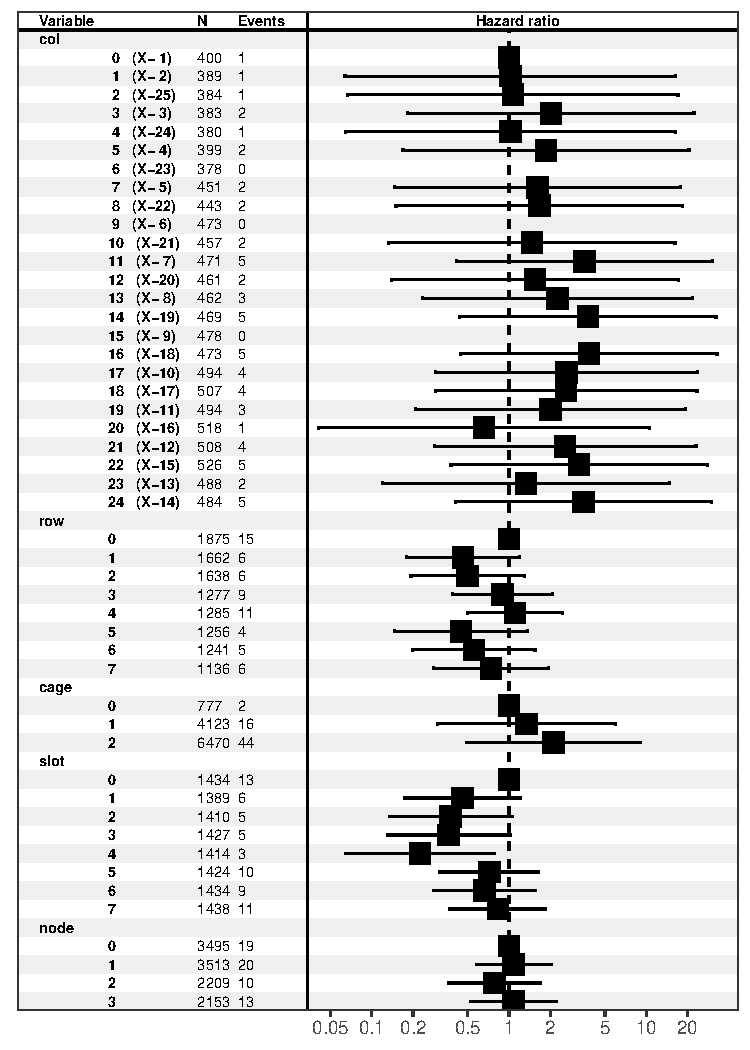
\includegraphics[width=\columnwidth]{figs/cox_n001.pdf}
  \caption{GPU hazard ratios from Cox regression model on {\tt new}
    batch.}
  \label{fig:cox-new}
\end{figure}

It appears that transport of cooling air provides a complete
explanation for relative differences in cage and node survival rates
in the old batch.  We reach this conclusion with reference to
Figure~\ref{fig:layout} and relative positions of cages and nodes
within a cabinet. Both cage and node differences in survival
probabilities can be explained by an inverse relationship with the
distance to the bottom of the cabinet, where cooling air is forced
through the cabinet to the top. The survival curves can be ordered
({\em cage 0, cage 1, cage 2}) in decreasing order of survival. As the
blades are placed vertically within the cabinet, pairs of nodes too
experience the same relationship with distance to the bottom, nodes 2
and 3 having lower failure rates than nodes 0 and 1.

Very few failures have occurred in the new batch and they are clearly
less prone to failure at the 2.5 year mark. There is a slight change
at the 3 year mark of cages 1 and 2 but it is also accompanied with a
rise in uncertainty and survival is still well above levels in the old
batch.

We don't see a ``bathtub curve'' phenomenon, in fact the opposite is
apparent in cages 1 and 2 of the old batch. The slope of the survival
curve is related to the hazard rate. There does not seem to be an
early ``infant mortality'' period nor a ``wearout'' phenomenon at the
end. Rather, we see a steeper slope (higher hazard rate) in the
middle, associated with the unexpected resistor failures.

To get more comparison power across the locations, we can use a
technique that in a sense averages over time. Cox proportional hazards
(CPH) regression analysis, can include covariates and estimates relative
risk averaged over time based on the covariates
\cite{Cox1972,Harrell2015}. The CPH regression function takes the form
\begin{displaymath}
  h(t) = h_0(t)e^{b_1 x_1 + b_2 x_2 \ldots b_k x_k},
\end{displaymath}
where $x_i$ are covariates, $h_0(t)$ is the {\em baseline hazard}, and
the $b_i$ are coefficients that measure the impact of the
covariates. The quantity $e^{b_i}$ is the hazard ratio (increased
average risk over baseline) for covariate $i$.

CPH is considered a semi-parametric model as there are no assumptions
about the shape of the baseline hazard function. Its strongest
assumption is that the hazards are proportional. There are a number of
tests for this, including graphical diagnostics in the \pkg{survminer}
package as well as checking that survival curves for categorical
covariates do not cross. We ran these diagnostics and concluded that
the hazards for our location categories are approximately
proportional. However, survival functions partitioned on {\em batch}
do cross and so we fit the model to the new and the old batches
separately. The results are presented in Figures~\ref{fig:cox-old}
and~\ref{fig:cox-new}.

We find that the average hazard ratios strongly correlate with
detailed nuances of the system cooling architecture.  The figures give
hazard ratios for each of the location variables, giving the ratio for
each level compared to its first (0) level (consequently the 0 level
is always 1). Due to the exponential nature of the CPH model, the
horizontal hazard ratio axis is on a log scale. The estimates include
uncertainty, which too is most reliably computed on a log scale (see,
for example, \cite{Ostrouchov88}). In the figures, we also include the
number of units, N, at risk and the number of events that occurred in
each category.

All the factors ({\em col, row, cage, slot, node}) in the old batch
are balanced with respect to the number of units at risk and
consequently nearly orthogonal (each level of a factor contains all
levels of the other factors) seemingly an almost ``designed''
experiment nature to this analysis. This is not the case for the new
batch, where the cage levels have very different numbers of units at
risk. But this also points out that even for the old batch the balance
holds only at the outset and as life proceeds, failing units are
replaced with new units and the balance degrades because failures are
location-dependent.

Our interpretation of correlation with details of the cooling system
comes mostly from the hazard ratios for the old batch. The new batch
has mot had many failure events and the uncertainty bars of nearly all
ratios include 1, which is no difference. In the old batch, we see
that {\em cage} has the strongest effect, putting the highest hazard
ratio on cage 2, which is consistent with lowest survivals in the KM
analysis earlier. Its ratio value near 20 has to be interpreted with
caution because it is a time averaged value on a log scale and suffers
from the degrading balance mentioned in the previous paragraph. This
aspect is not captured by the uncertainty, which accounts for the
randomness of the failures and not for the geometric time averaging
\cite{coxhazardinterpret}. Consequently, we interpret the pattern of
relative hazards rather than actual ratio magnitudes. More in-depth
analysis with penalized estimation methods like \cite{bender2019} can
take such balance issues in the exposure history into account and
provide time-dependent hazard estimates.

In addition to the strong {\em cage} and {\em node} hazard rate
differences that increase with distance from the bottom of the
cabines, seen in both KM and CPH results, there is a weaker but
peculiar pattern in the {\em row} and {\em col} hazard rates. The
different behavior in {\em col} 0-11 from {\em col} 12-24 is likely
due to separate supply lines of chilled water to the two sets. While
the temperature was a consistent 42$^\circ$F, there may have been
minor flow or pressure differences. But the interleaving pattern of
the first set is still a mystery. We also have yet to explain the
apparent row effects. A very minor airflow effect across slots also
seems to be present as it mimics faster airflow for the middle slots.


%%%%%%%%%%%%
% Discussion
%%%%%%%%%%%%
% !TEX root = main.tex
%%%%%%%%%%%%%%%%%%%%%%%%%%%%%%%%%%%%%%%%%%%%%%%%%%%%%%%%%%%%%%%%%%%%%%%%%%%%%%%%
% Conclusions
%%%%%%%%%%%%%%%%%%%%%%%%%%%%%%%%%%%%%%%%%%%%%%%%%%%%%%%%%%%%%%%%%%%%%%%%%%%%%%%%
\section{\rev{Conclusions}}
\label{section:discussion}

\rev{The failure rates of the old batch are not matched by the new
  batch nor by experience at other facilities with the same type of
  GPU components, making this an unexpected event that had
  considerable impact on operations and on availability of the
  system. On a positive but ironic note, the corrosion process in the
  failing resistors made the specific GPU batch act as sensitive
  instruments for obtaining cummulative trend information from
  component heat dynamics and provided lessons learned. Here we
  dicsuss the conclusions we can draw from the experience on
  mitigation, which keeps the system operating at an acceptable level
  and possibly even restores some of the lost capability, and on
  long-term planning, which addresses such scenarios in
  future-generation supercomputers.}

%%%%%%%%%%%%
% Mitigation
%%%%%%%%%%%%
\subsection{Mitigation}
\label{section:mitigation}

In Titan, the mitigation component included replacing about 11,000 GPUs and
changing the job scheduling strategy~\cite{8665764}. Replacing about 59\% of
Titan's 18,688 GPUs helped to improve productivity by restoring some of the lost
capability, but it was a costly and time-consuming effort. Changing the job
scheduling strategy to run larger jobs on more reliable and smaller jobs on less
reliable nodes played a crucial role in maintaining productivity at reduced
capability. However, jobs running on larger portions of the system, utilizing
most or all of its resources, were still impacted by the failing GPUs and
corresponding low system MTBF.

The options of replacing failed components and employing reliability-aware
resource management may not be available or be cost effective for other
supercomputing centers dealing with similar unexpected reliability issues.
%
Replacement components may not be readily available and may have to be
manufactured, which can be impossible for a technology that is no longer supported
by the original manufacturer. Experienced errors or failures may be caused by
software, which can be difficult to fix if the software itself or the deployed
version is no longer supported by the vendor.

There is also a financial aspect, such as a service contract and/or warranty
expiration and the operational budget of a supercomputing center not having
significant funds for replacement/reengineering costs or a manufacturer or
vendor not paying for them.
%
There is additionally the time and financial cost for root-cause analysis and
for developing a hardware and/or software mitigation strategy in the first place.
Fixing a problem requires finding and understanding it, which can be difficult 
in today's complex systems and may require knowledge that only the original 
manufacturer or vendor possesses.

Reliability-aware resource scheduling also has its limitations, as the network
architecture needs to be taken into account. Titan's 3D torus network creates
certainly more challenges for efficient job allocations, than the fat tree
network of Titan's successor, Summit~\cite{olcf:summit}. Nodes associated with
the same job need to be close to each other on the network for maximum
application performance. Also, node outages or less reliable nodes within a
tight group of reliable nodes create resource allocation
holes. Separating two lower nodes in each cage 0 on Titan would not
create a contiguous partition, yet this group would be the most
reliable in 2016 as was shown in the preceeding section.
%
Alternatively, partially or completely replacing the aging and failing
supercomputer with a new system, even if this solution offers less capability,
may be more cost effective in the end.

Other mitigation components for Titan included matching the checkpointing
interval of applications with the system's current
reliability~\cite{bautista-gomez16reducing, 6903564}. The experienced issue here
was the lack of automated communication of system reliability information and
the lack of flexibility in application-level checkpoint/restart implementations.
Constantly measuring and reporting current system reliability is not an automated
real-time task in many currently deployed supercomputers. Applications are
typically not designed to skip a checkpoint when system reliability is good or
take more frequent checkpoints when system reliability is getting worse.

%%%%%%%%%%%%%%%%%%%%
% Long-term Planning
%%%%%%%%%%%%%%%%%%%%
\subsection{Long-term Planning}
\label{section:planning}

The long-term planning component is one of the biggest lessons learned from the
Titan reliability experience. Today's supercomputers are designed to deal with
expected reliability issues. However, history has shown~\cite{geist12kill} that
unexpected reliability issues do occur and do have a significant impact. Vendors
and manufacturers obviously can not mitigate against all possible reliability
threats, however, a resilience strategy is needed for future-generation systems
that is able to deal with emerging unexpected reliability threats in a
reasonable and cost effective way. In addition to mitigation, better support for
automated real-time reliability monitoring and reporting is needed, including
for root-cause analysis.

Supercomputer center policies regarding reliability monitoring, resource
allocation and checkpointing strategies need to be powerful and flexible enough
to facilitate mitigation for such unexpected reliability threats. System
acquisition contracts may need to include performance requirements for degraded
operation, such as a certain percentage of performance capability if the MTBF
drops by an order of magnitude.

\rev{The experienced reliability issues with Titan had a direct impact on the
development and deployment of Titan's successor, Summit, and even on Summit's
successor, Frontier. As a result, more and better monitoring data is already
collected on Summit. NVIDIA's GPU management and monitoring software has been
significantly improved. Temperature monitoring has been significantly improved
as well.}

%%%%%%%%%%%%%%%%%
% Acknowledgments
%%%%%%%%%%%%%%%%%
\doubleblind{% !TEX root = main.tex
%%%%%%%%%%%%%%%%%%%%%%%%%%%%%%%%%%%%%%%%%%%%%%%%%%%%%%%%%%%%%%%%%%%%%%%%%%%%%%%%
% Acknowledgments
%%%%%%%%%%%%%%%%%%%%%%%%%%%%%%%%%%%%%%%%%%%%%%%%%%%%%%%%%%%%%%%%%%%%%%%%%%%%%%%%
\section{Acknowledgments}
\label{section:acknowledgments}

This work was supported by the U.S. Department of Energy, Office of Science,
Office of Advanced Scientific Computing Research, program managers Robinson Pino
and Lucy Nowell, under contract number DE-AC05-00OR22725. \fix{Add any additional
funding acknowledgements}}{}

%%%%%%%%%%%%%%%%%%%%%%%%%%%%%%%%%%%%%%%%%%%%%%%%%%%%%%%%%%%%%%%%%%%%%%%%%%%%%%%%
% References
%%%%%%%%%%%%%%%%%%%%%%%%%%%%%%%%%%%%%%%%%%%%%%%%%%%%%%%%%%%%%%%%%%%%%%%%%%%%%%%%
\bibliographystyle{IEEEtran}
\bibliography{refs}

%%%%%%%%%%%%%%%%%%%%%%%%%%%%%%%%%%%%%%%%%%%%%%%%%%%%%%%%%%%%%%%%%%%%%%%%%%%%%%%%
% End of Document
%%%%%%%%%%%%%%%%%%%%%%%%%%%%%%%%%%%%%%%%%%%%%%%%%%%%%%%%%%%%%%%%%%%%%%%%%%%%%%%%
\end{document}
